\documentclass[main_brownies.tex]{subfiles}
\begin{document}
\graphicspath{ {Figures/}{Schemes/} } % graphics path for two folders: \Figures and \Schemes
\newrefsection[Instructions/References_Instructions] %% begin new reference section with the .bib file for this chapter

%% an if-else statement for inserting an empty page when necessary
%% to make sure chapter image page is to the left of the chapter title page
\checkoddpage
\ifoddpage
\newpage\thispagestyle{empty}
\mbox{}
\newpage

\includepdf[pages={-}]{Image_notepad.pdf} % can change to a different image
\else

\includepdf[pages={-}]{Image_notepad.pdf} % can change to a different image
\fi

\chapter[Instructions]{Style and Printing Considerations} %% the [short title] will end up in the TOC as well
	
\begin{abstract}
	Text that is already italic (for example in the abstract) and again italicized. Consider 
	\begin{LTXexample}[pos=b,preset=\centering,width=0.5\linewidth]
		\textit{text} and \emph{text}
	\end{LTXexample}
\end{abstract}

\section{To do}
\begin{itemize}
	\item \textcolor{red}{ADD THE USEFUL NOTES AND SUCH FROM THE OTHER CHAPTERS HERE TOO.}
	\item \textcolor{red}{ADD rest of the links as references}
	\begin{itemize}
		\item Subfigures: https://latex-tutorial.com/subfigure-latex/
	\end{itemize}
	\item add small bit of instructions on how to make the firstpage and titlepage (refer to .tex files)
	\item recommend to use \verb*|\qty{}{}| and \verb*|\unit{}| any time you can. For example, also to indicate temperature or an angle: \qty{50}{\degree C} and \qty{180}{\degree} backscattering setup
\end{itemize}

\section{General}
\begin{itemize}
	\item It can be necessary \textbf{to compile your document twice} for certain changes to take effect, in particular those concerning labels (floats, references, etc.) that are stored in auxiliary files, so keep this in mind when trying to find out whether an adjustment in the code has had the desired result in the output.
	\item The symbol \verb*|~| is used as a "glue" that sticks two characters to each other such that there will not be a line break made between them. It is used, for example, when referring to floats: Figure~\ref{fig:left}.
	\item To make an en-dash (--), type \verb*|--|
	\item To make an em-dash (---), use \verb*|---|
	\item see previous Chapters: \textbf{add useful instructions, and refer to sections in the Chapters for examples that possibly have more details.}
\end{itemize}

The package \verb*|extdash| provides commands for unbreakable dashes and options for hyphenations. To prevent hyphenation of a word that does not contain hyphens already, use the command \verb*|hyphenation{thiswordwilllooklikethis}| (in the pre\=/amble). The same command can be used to indicate where to allow hyphenation, e.g., \verb*|hyphenation{so-called}|.
It is recommended to add the option for use of shortcuts: \verb*|\RequirePackage[shortcuts]{extdash}|. The commands for unbreakable dashes are:
\begin{Verbatim}
	\=/ hyphen (still allows hyphenation between other syllables)
	\== en-dash
	\=== em-dash
\end{Verbatim}

\section{Making Macros}
It can be very useful to make your own macros (a.k.a. shortcuts/hotkeys) for commonly used commands, e.g., \verb|\textsubscript| and \verb|\textmu|, in the same way that those for \textit{italic} (\verb|Ctrl+i|) and \textbf{bold-face} (\verb|Ctrl+b|) work.

\section{Headers and Footers}
The package \verb*|fancyhdr| has a few default options. Importantly, the thickness of the headrule (\verb*|headrulewidth|) is 0.4pt by default. The thicknesses of the footrules and headrules can be adjusted like so:
\begin{Verbatim}[breaklines=true]
	\renewcommand{\footrulewidth}{0.4pt} % to add footrule in mainmatter. headrulewidth is defined in the package fancyhdr: default is 0.4pt
	\renewcommand*\headrulewidth{0pt}
\end{Verbatim}

\section{Figures}
Define \verb*|\graphicspath| per \verb*|\subfile| (\textit{i.e.}, Chapter) like so:\cite{GraphicsPathSubfiles}
\begin{Verbatim}[breaklines=true, breakanywhere=true]
	\graphicspath{ {Figures/}{Schemes/} }
\end{Verbatim}

\subsection{Figures from python}
We decided: pdf's because they are vector images (look better) and have relatively small file sizes, depending on the amount of data inside. Pdf's made in python are in RGB, this is easily changed in AdobeIllustrator: open pdf in illustrator, change File/Document Color Mode to CMYK and save again. For printing, CMYK is recommended. Also you can use illustrator to change the size of the figure or artboard or rearrange subplots a little bit. Oddly enough: png's and pdf's made in python and converted to CMYK in illustrator are slightly different in colour so always be consistent in your file extensions. 

\subsection{How to make new floats}
\begin{Verbatim}[breaklines=true, breakanywhere=true]
	\RequirePackage{float}
	\RequirePackage{newfloat}
	\DeclareFloatingEnvironment[fileext=los, name=Scheme, placement=htbp]{scheme}
	\DeclareFloatingEnvironment[fileext=los, name=Figure, placement=htbp]{figureSI} % new float figureSI
	\DeclareFloatingEnvironment[fileext=los, name=Scheme, placement=htbp]{schemeSI} % new float schemeSI
	\DeclareFloatingEnvironment[fileext=los, name=Table, placement=htbp]{tableSI} % new float tableSI
	
	\addto{\captionsenglish}{\renewcommand{\thefigureSI}{S\arabic{figureSI}}} % label Figure S#"
	\addto{\captionsenglish}{\renewcommand{\theschemeSI}{S\arabic{schemeSI}}} % label Scheme S#"
	\addto{\captionsenglish}{\renewcommand{\thetableSI}{S\arabic{tableSI}}} % label Table S#"
\end{Verbatim}

\subsection{Align figures}
There is several ways of scaling figures but I think most of them are relative to the page so best to start with all figures of the same width or scale them according to original size

\subsubsection{Location on page}
Useful options and commands:
\begin{Verbatim}
	[htbp]
	\FloatBarrier
	\clearpage
\end{Verbatim}
Everything we want to say about this is described well by Rob J. Hyndman.\cite{Hyndsight}\\

\noindent\dotfill\textit{Copied directly from his webpage:}\dotfill\\
Use the placement options: h, t, b and p. For example \verb*|\begin{figure}[htb]| causes LaTeX to try to fit the float “here”, or at the “top” of the current page (or the next page), or at the “bottom” of the current page (or the next page). If “p” is specified, it will allow the float to take a whole page to itself. You can’t specify only “h” as that is too restrictive, and LaTeX will automatically change it to “ht”. The default setting is “tbp”.
	
One of the reasons that the floats won’t go where you want them is that there are a lot of constraints on where they can go. The main ones are:

%\begin{center}
\begin{adjustbox}{width=1\textwidth}
	\begin{tabular}{ccc}
		\hline
		Counter&&Default\\
		\hline
		topnumber&maximum number of floats at top of page&2\\
		bottomnumber&maximum number of floats at bottom of page&1\\
		totalnumber&maximum number of floats on a page&3\\
		\hline
		Command&&\\
		\hline
		\verb*|\topfraction|&maximum fraction of page for floats at top&0.7\\
		\verb*|\bottomfraction|&maximum fraction of page for floats at bottom&0.3\\
		\verb*|\textfraction|&minimum fraction of page for text&0.2\\
		\verb*|\floatpagefraction|&minimum fraction of floatpage that should have floats&0.5\\
		\hline
	\end{tabular}
\end{adjustbox}
%\end{center}

These can all be changed individually. But it is often easier to add ! before the placement options, thus forcing LaTeX to ignore most of these contraints. For example, I often use \verb*|\begin{figure}[!htb]|. If you want to change the defaults, the following values give reasonable results:
\begin{verbatim}
	\setcounter{topnumber}{2}
	\setcounter{bottomnumber}{2}
	\setcounter{totalnumber}{4}
	\renewcommand{\topfraction}{0.85}
	\renewcommand{\bottomfraction}{0.85}
	\renewcommand{\textfraction}{0.15}
	\renewcommand{\floatpagefraction}{0.7}
\end{verbatim}
The \verb*|\clearpage| command starts a new page and inserts all floats that have not yet appeared before continuing. This can leave a bad page break, so a useful alternative is to use the \verb*|afterpage| package, and then insert \verb*|\afterpage{\clearpage}| which will put all the floats at the end of the current page.

A very useful package is \verb*|placeins|. This provides the command \verb*|\FloatBarrier| which causes all unprocessed floats to be processed at that point, but does not start a new page unless it is necessary. To keep floats in the sections in which they were included, use \verb*|\RequirePackage[section]{placeins}|. This silently puts a \verb*|\FloatBarrier| command before each section. There are other options explained in the \verb*|placeins| documentation.
		
Another useful package is \verb*|flafter|. This causes floats to always appear after their placement in the document.
		
If you really don’t want LaTeX to move your float at all, then use the \verb*|float| package with the command \verb*|\restylefloat{figure}| in the preamble. This allows you to specify \verb*|[H]| as the position parameter which means "Here and only Here". However, this often gives bad page breaks.\\

\noindent\dotfill

\subsubsection{Minipage}
The \verb*|minipage| environment does not require a separate package.

\begin{figure}[tbh]
%	\centering
	\begin{minipage}[t]{0.5\textwidth}
		
\includegraphics[width=\textwidth]{6colors.pdf}
		\captionof{figure}{Caption of figure on the left}
		\label{fig:left}    
	\end{minipage}%
%	\hspace{0.05\textwidth}
	\hfill
	\begin{minipage}[t]{0.5\textwidth}
%		\centering
		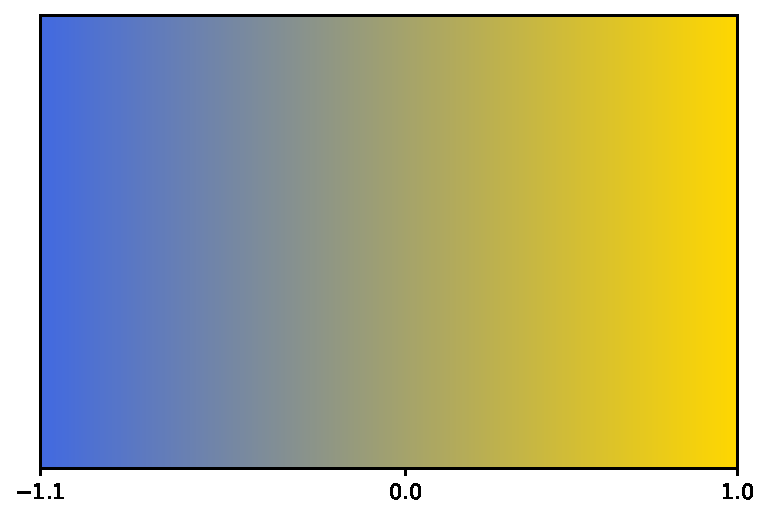
\includegraphics[width=\textwidth]{test3.pdf}
		\captionof{figure}{Caption of figure on the right}
		\label{fig:right}
	\end{minipage}%
%	\caption{Shared caption for both figures (not recommended but optional).}
\end{figure}%
Minipages are one way to arrange figures next to each other, or for example when you want to add separate captions to two figures. You can also have a shared caption for two figures, see example.

\subsubsection{Subfigures}
To make a figure consisting of subfigures, each with their own respective subcaption, requires the use of the package \verb*|subcaption|. See Figure~\ref{fig:subfigures} for an example. Referring to the individual subfigures is also possible, e.g., see Figure~\ref{fig:subfig_a}.

\begin{figure}[htb]
	\centering
	\begin{subfigure}[b][][c]{0.45\textwidth}
		\centering
		
\includegraphics[width=\textwidth]{Subfigures/Subfigure_a}
		\caption{Caption of Subfigure a.}
		\label{fig:subfig_a}
	\end{subfigure}
	\hfill
	\begin{subfigure}[b][][c]{0.45\textwidth}
		\centering
		
\includegraphics[width=\textwidth]{Subfigures/Subfigure_b}
		\caption{Caption of Subfigure b.}
		\label{fig:subfig_b}
	\end{subfigure}
	\caption{Caption of whole Figure.}
	\label{fig:subfigures}
\end{figure}

\section{Tables}
Here is a list of useful packages for tables:
\begin{Verbatim}[breaklines=true]
	\RequirePackage{multirow} % to merge cells in tables
	\RequirePackage{makecell} % to insert linebreak in cells in tables
	\RequirePackage{array} % extra options and for better working of tabular and array
	\RequirePackage{adjustbox} % to resize tables
	\RequirePackage{tabularx} % tabularx readjusts column widths to fill appointed size (x\textwidth)
	\RequirePackage{boldline} % to make thicker lines % https://tex.stackexchange.com/questions/314882/tabular-thicker-lines
	\RequirePackage{adjustbox} % Limit table
	\RequirePackage{colortbl} % colors in tables.
	\RequirePackage{rotating} % table rotation
	\RequirePackage{supertabular} % allows two-column tables for when they are too long for one page
	\RequirePackage{longtable} % allows multi-page tables
	\RequirePackage{csvsimple} % to make table from .csv (not needed for simple tables)
\end{Verbatim}

\section{Captions}
The style of the figure captions is set using the package \verb*|caption| and its associated command \verb*|\captionsetup| (\emph{see below}).

\subsection{Layout of captions}
The style of the caption can be changed to your liking:
\begin{itemize}
	\item indentation
	\item font family and type (e.g., boldface, sans serif)
	\item separator (. , ; :)
	\item and more!
\end{itemize}

Here is an example of a caption setup with certain options specified:
\begin{Verbatim}[breaklines=true, breakanywhere=true]
	\captionsetup{singlelinecheck=off,format=plain,indention=0.0cm,labelsep=colon,labelfont=bf,font={sf,small}}
\end{Verbatim}

\section{Indentation of text}
Paragraphs can start with an indentation or not depending on whether you want that or not. Oddly enough, there is a difference between a double empty line and a double backslash.

This is one line of text after a double empty line.\\
This is another line of text but now after a double backslash.

The document class is set in such a way that the first paragraph of a section does not start with an indent, but other paragraphs after do, using the option \verb*|noindentafter| in the package \verb*|titlesec|, like so:
\verb*|\RequirePackage[noindentafter]{titlesec}|

\subsection{Paragraph spacing}
The package \verb|parskip| can be used to adjust the paragraph spacing:  The other values are:
\begin{itemize}
	\item The value of \verb|\parindent| can be set via the \texttt{indent} option. It is now \texttt{\the\parindent}.
	\item \verb|\baselineskip| is \texttt{\the\baselineskip}
	\item \verb|\parskip| can be set via the \texttt{skip} option. Its value is \texttt{\the\parskip}
	\item \verb|\tocskip| can be set via the \texttt{tocskip} option. This should set the paragraph spacing in the TOC, but I have not been able to get it to work (the TOC spacing just uses the normal \verb|\parskip|...)
\end{itemize}

\section{Miscellaneous Environments and Commands}
\subsection{A Command for an Experimental Procedure: synth}
Defined a command \verb*|\synth| with 5 (optional) arguments all inside a minipage (such that no experimental procedure spreads over two pages). The input fields are: title; image; text; NMR; HRMS (but these are optional and can be adjusted/appended as well).
The code for \verb*|\includegraphics| is simplified: it is now only necessary to input the name of the image file -- the rest of the code is included in \verb*|\synth|.

And another important feature: using the argument \verb*|scale=| instead of setting the width (with \verb*|width=|) for \verb*|\includegraphics| makes sure that the images of the molecules retain their relative dimensions -- the molecules share the same ratio but have various heights and widths depending on their substitution pattern.
Parameters in \verb*|\synth| that can be adjusted to achieve the desired result are:
\begin{itemize}
	\item The size of the \verb*|wrapfigure| and hereby the amount of whitespace around the molecules
	\item The scaling factor of the image that is included with \verb*|\includegraphics[scale=<value>]|
	\item The vertical whitespace between the molecule and the title by the command \verb*|\vspace*{-<value>\baselineskip}| which removes a certain amount of vertical space (note the \textit{minus} sign)
\end{itemize}
These parameters are in this part of the code for \verb*|\synth| which can be found above:
{\small
\begin{verbatim}
	-----------------------------------
	\begin{wrapfigure}{l}{0.20\textwidth}% -- Change the value of the number before \textwidth
		\centering
		\vspace*{-0.75\baselineskip} -- Change the magnitude of \baselineskip
		\includegraphics[scale=0.15]{#2} -- The scaling factor of the image
		%			\vspace*{-\baselineskip}%
	\end{wrapfigure}\small{#3} %
	-----------------------------------
\end{verbatim}
}

\section{Referencing}
This Biblatex cheat sheet is handy.\cite{BiblatexCheatSheet}

For authors with last names that are two words or consist of two parts -- use either of these options in the .bib file:\cite{BibTwowordlastname}
\begin{itemize}
	\item De Gaulle, Charles
	\item Charles {De Gaulle}
\end{itemize}

For each separate chapter, it is recommended to use a separate \verb*|refsection| as well, for example using the command \verb*|\newrefsection["bibfilename"]| at the start of the subfile (Chapter) .tex file. For example, for Chapter~1 of this document, we added: \verb*|\newrefsection[Chapter_1/References_Chapter_1]|. See Biblatex documentation for detailed information.\cite{BiblatexDocumentation}

%%%==== References ====%%%

{\raggedright
	\printbibliography} %% use to loosen restrictions on justification for References section. 
%% If \raggedright is not used, there will be many warnings for overfull hboxes

\end{document}
